% §6 Design Lever Taxonomy
Having established the latency floor and its compounding behaviour for multi-step agents,
we now classify the engineering strategies used to reduce the perceived silence gap.
A key distinction emerges: some strategies reduce the irreducible floor $\Lambda^*$
(structural fixes), while others reduce only the reducible component $\lambda_i^r$
or mask the gap perceptually without changing the floor at all.

Figure~\ref{fig:design_levers} summarises the seven strategies across five dimensions:
the pipeline stage targeted, the latency component addressed, the headroom recovered,
and whether the strategy reduces $\Lambda^*$ itself.

\begin{figure}[t]
  \centering
  \resizebox{\linewidth}{!}{%
    % Fig 4: Design lever taxonomy matrix
% Seven strategies x five columns; explicit node placement to avoid foreach-tuple errors.
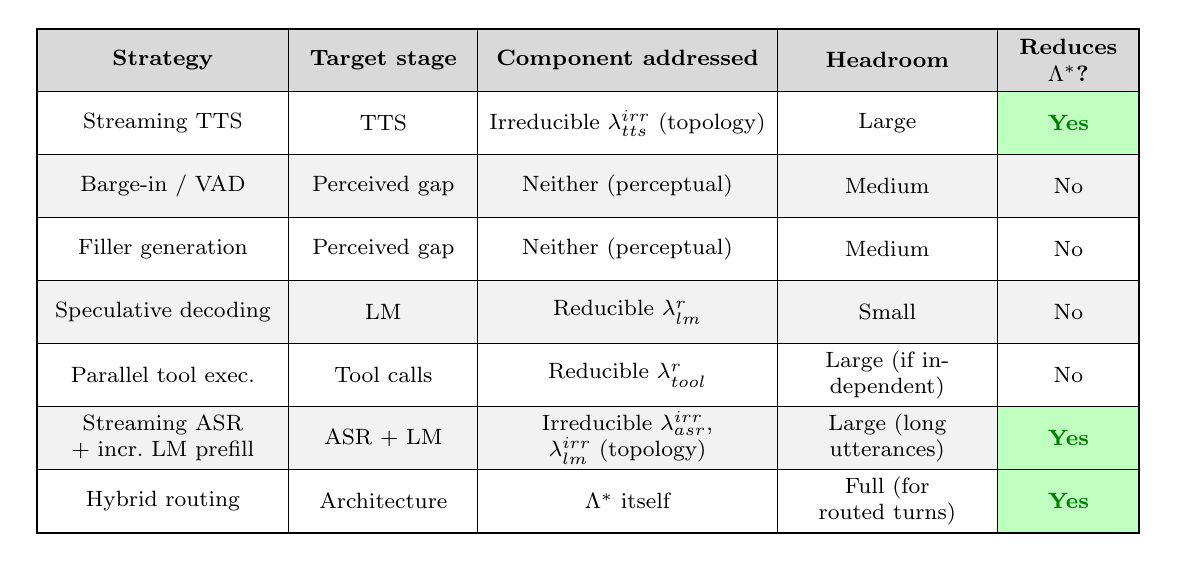
\begin{tikzpicture}[font=\footnotesize]

% Geometry (unitless numbers; appended with "cm" at each use)
\def\rh{0.80}  % row height (cm)
\def\ca{3.2}   % col 1 width: Strategy
\def\cb{2.4}   % col 2 width: Target stage
\def\cc{3.8}   % col 3 width: Component addressed
\def\cd{2.8}   % col 4 width: Headroom
\def\ce{1.8}   % col 5 width: Reduces Lambda*?

% Derived x-positions of left edges of each column
\pgfmathsetmacro{\xA}{0}
\pgfmathsetmacro{\xB}{\xA+\ca}
\pgfmathsetmacro{\xC}{\xB+\cb}
\pgfmathsetmacro{\xD}{\xC+\cc}
\pgfmathsetmacro{\xE}{\xD+\cd}
\pgfmathsetmacro{\xF}{\xE+\ce}

% Derived x-positions of centres of each column
\pgfmathsetmacro{\mA}{\xA+\ca/2}
\pgfmathsetmacro{\mB}{\xB+\cb/2}
\pgfmathsetmacro{\mC}{\xC+\cc/2}
\pgfmathsetmacro{\mD}{\xD+\cd/2}
\pgfmathsetmacro{\mE}{\xE+\ce/2}

% ── HEADER ROW (y = 0 to +\rh) ──────────────────────────────────────────────
\fill[gray!30] (\xA,0) rectangle (\xF,\rh);
\node[align=center, font=\footnotesize\bfseries, text width=\ca cm] at (\mA,{0.5*\rh}) {Strategy};
\node[align=center, font=\footnotesize\bfseries, text width=\cb cm] at (\mB,{0.5*\rh}) {Target stage};
\node[align=center, font=\footnotesize\bfseries, text width=\cc cm]
  at (\mC,{0.5*\rh}) {Component addressed};
\node[align=center, font=\footnotesize\bfseries, text width=\cd cm] at (\mD,{0.5*\rh}) {Headroom};
\node[align=center, font=\footnotesize\bfseries, text width=\ce cm]
  at (\mE,{0.5*\rh}) {Reduces $\Lambda^*$?};

% ── Helper macro: row shading ────────────────────────────────────────────────
% Row 1: y from 0 down to -\rh, row 2: -\rh to -2*\rh, etc.

% Row 1 — Streaming TTS (YES — highlighted green for last cell)
\fill[white]     (\xA,{-0*\rh}) rectangle (\xF,{-1*\rh});
\fill[green!25]  (\xE,{-0*\rh}) rectangle (\xF,{-1*\rh});
\node[align=center, text width=\ca cm]
  at (\mA,{-0.5*\rh}) {Streaming TTS};
\node[align=center, text width=\cb cm]
  at (\mB,{-0.5*\rh}) {TTS};
\node[align=center, text width=\cc cm]
  at (\mC,{-0.5*\rh}) {Irreducible $\lambda_{tts}^{irr}$ (topology)};
\node[align=center, text width=\cd cm]
  at (\mD,{-0.5*\rh}) {Large};
\node[align=center, font=\footnotesize\bfseries, color=green!50!black, text width=\ce cm]
  at (\mE,{-0.5*\rh}) {Yes};

% Row 2 — Barge-in / VAD
\fill[gray!10]   (\xA,{-1*\rh}) rectangle (\xF,{-2*\rh});
\node[align=center, text width=\ca cm]
  at (\mA,{-1.5*\rh}) {Barge-in / VAD};
\node[align=center, text width=\cb cm]
  at (\mB,{-1.5*\rh}) {Perceived gap};
\node[align=center, text width=\cc cm]
  at (\mC,{-1.5*\rh}) {Neither (perceptual)};
\node[align=center, text width=\cd cm]
  at (\mD,{-1.5*\rh}) {Medium};
\node[align=center, text width=\ce cm]
  at (\mE,{-1.5*\rh}) {No};

% Row 3 — Filler generation
\fill[white]     (\xA,{-2*\rh}) rectangle (\xF,{-3*\rh});
\node[align=center, text width=\ca cm]
  at (\mA,{-2.5*\rh}) {Filler generation};
\node[align=center, text width=\cb cm]
  at (\mB,{-2.5*\rh}) {Perceived gap};
\node[align=center, text width=\cc cm]
  at (\mC,{-2.5*\rh}) {Neither (perceptual)};
\node[align=center, text width=\cd cm]
  at (\mD,{-2.5*\rh}) {Medium};
\node[align=center, text width=\ce cm]
  at (\mE,{-2.5*\rh}) {No};

% Row 4 — Speculative decoding
\fill[gray!10]   (\xA,{-3*\rh}) rectangle (\xF,{-4*\rh});
\node[align=center, text width=\ca cm]
  at (\mA,{-3.5*\rh}) {Speculative decoding};
\node[align=center, text width=\cb cm]
  at (\mB,{-3.5*\rh}) {LM};
\node[align=center, text width=\cc cm]
  at (\mC,{-3.5*\rh}) {Reducible $\lambda_{lm}^r$};
\node[align=center, text width=\cd cm]
  at (\mD,{-3.5*\rh}) {Small};
\node[align=center, text width=\ce cm]
  at (\mE,{-3.5*\rh}) {No};

% Row 5 — Parallel tool execution
\fill[white]     (\xA,{-4*\rh}) rectangle (\xF,{-5*\rh});
\node[align=center, text width=\ca cm]
  at (\mA,{-4.5*\rh}) {Parallel tool exec.};
\node[align=center, text width=\cb cm]
  at (\mB,{-4.5*\rh}) {Tool calls};
\node[align=center, text width=\cc cm]
  at (\mC,{-4.5*\rh}) {Reducible $\lambda_{tool}^r$};
\node[align=center, text width=\cd cm]
  at (\mD,{-4.5*\rh}) {Large (if independent)};
\node[align=center, text width=\ce cm]
  at (\mE,{-4.5*\rh}) {No};

% Row 6 — Streaming ASR + Incremental LM prefill (YES — highlighted green)
\fill[gray!10]   (\xA,{-5*\rh}) rectangle (\xF,{-6*\rh});
\fill[green!25]  (\xE,{-5*\rh}) rectangle (\xF,{-6*\rh});
\node[align=center, text width=\ca cm]
  at (\mA,{-5.5*\rh}) {Streaming ASR + incr.\ LM prefill};
\node[align=center, text width=\cb cm]
  at (\mB,{-5.5*\rh}) {ASR + LM};
\node[align=center, text width=\cc cm]
  at (\mC,{-5.5*\rh}) {Irreducible $\lambda_{asr}^{irr}$, $\lambda_{lm}^{irr}$ (topology)};
\node[align=center, text width=\cd cm]
  at (\mD,{-5.5*\rh}) {Large (long utterances)};
\node[align=center, font=\footnotesize\bfseries, color=green!50!black, text width=\ce cm]
  at (\mE,{-5.5*\rh}) {Yes};

% Row 7 — Hybrid routing (YES — highlighted green)
\fill[white]     (\xA,{-6*\rh}) rectangle (\xF,{-7*\rh});
\fill[green!25]  (\xE,{-6*\rh}) rectangle (\xF,{-7*\rh});
\node[align=center, text width=\ca cm]
  at (\mA,{-6.5*\rh}) {Hybrid routing};
\node[align=center, text width=\cb cm]
  at (\mB,{-6.5*\rh}) {Architecture};
\node[align=center, text width=\cc cm]
  at (\mC,{-6.5*\rh}) {$\Lambda^*$ itself};
\node[align=center, text width=\cd cm]
  at (\mD,{-6.5*\rh}) {Full (for routed turns)};
\node[align=center, font=\footnotesize\bfseries, color=green!50!black, text width=\ce cm]
  at (\mE,{-6.5*\rh}) {Yes};

% ── GRID LINES ───────────────────────────────────────────────────────────────

% Outer border
\draw[thick] (\xA,\rh) rectangle (\xF,{-7*\rh});

% Horizontal row separators (between header and row 1, and between data rows)
\foreach \row in {0,1,2,3,4,5,6} {
  \draw (\xA,{-\row*\rh}) -- (\xF,{-\row*\rh});
}

% Vertical column separators (inner only)
\foreach \x in {\xB,\xC,\xD,\xE} {
  \draw (\x,\rh) -- (\x,{-7*\rh});
}

\end{tikzpicture}
%
  }
  \caption{Design lever taxonomy.
           Streaming TTS, streaming ASR with incremental LM prefill, and hybrid routing
           (highlighted green) reduce the irreducible latency floor $\Lambda^*$ itself.
           The remaining four strategies target reducible components or provide
           perceptual masking without structural impact on the floor.}
  \label{fig:design_levers}
\end{figure}

\subsection{Streaming Text-to-Speech}

Standard TTS systems require the complete response text before generating audio
\citep{shen2018natural}.
Streaming TTS begins audio generation after receiving a short prefix of the response ---
typically the first sentence or a fixed number of tokens.
This converts $\lambda_{tts}$ from a sequential dependency on the full LM output into
a dependency on only the first output tokens,
reducing $\lambda_{tts}^{irr}$ to the latency required to synthesise the first audio frame
from the first text tokens.
Streaming TTS therefore reduces $\Lambda^*$ directly and is a structural fix.
The tradeoff is that prosody planning across the full response is limited,
and audio quality may be lower for very short initial segments.

\subsection{Barge-In Detection}

Barge-in detection allows the agent to detect when the user begins speaking during
agent audio playback and to interrupt its own response immediately.
This does not reduce the silence gap for any individual turn where the user waits,
but it reduces the \emph{effective} silence gap by allowing the user to take the floor
before the agent has finished speaking.
Voice activity detection systems \citep{raux2008optimizing} provide the acoustic signal
for barge-in detection.
Barge-in is a perceptual patch: it masks the silence gap for turns where the user
interrupts early, but does not reduce $\Lambda^*$ for turns where the user waits for
the agent to finish.

\subsection{Filler Generation}

Filler generation plays a brief auditory cue (``hmm'', ``let me check'', ``one moment'')
immediately after ASR completes, before the LM response is ready.
This reduces the \emph{perceived} silence gap by replacing silence with an
acknowledgement signal.
Psycholinguistically, fillers signal that the conversational floor is held and
processing is underway \citep{levinson2015timing},
reducing the face-threatening interpretation of long gaps.
Filler generation does not reduce $\Lambda^*$:
the LM response must still complete before audio response begins,
and the filler audio is generated by a separate, lightweight model running in parallel
with the primary LM.
It is a perceptual patch with no structural impact on the latency floor.

\subsection{Speculative Decoding}

Speculative decoding \citep{leviathan2023fast} uses a small draft model to propose
candidate tokens that are verified in parallel by the full model,
reducing wall-clock time per generated token.
Applied to the LM stage, this reduces $\lambda_{lm}^r$ (the reducible component of LM latency)
but does not reduce $\lambda_{lm}^{irr}$,
since the prefill cost is determined by input context length
and not by token generation speed.
The practical headroom is modest: speculative decoding typically achieves 2--3$\times$
speedup on the decode phase,
with negligible effect on time-to-first-token for short responses.

\subsection{Parallel Tool Execution}

When a $k$-step ReAct agent issues tool calls that are \emph{independent} of each other
(i.e., no data dependency exists between them),
those calls can be executed in parallel rather than sequentially.
This replaces the sequential sum $(k-1) \cdot \lambda_{tool}$
with $\max_j(\lambda_{tool,j})$ in the silence gap expression,
a significant reduction for agents with many parallel-executable tool calls.
However, this strategy addresses only the reducible tool-call component;
the irreducible floor of the LM reasoning steps remains unchanged.
For tool calls with data dependencies, parallelism is not applicable.

\subsection{Streaming ASR with Incremental LM Prefill}

Streaming ASR systems---RNN-T \citep{graves2012sequence}, CTC-based streaming architectures
\citep{yao2021wenet}, and adapted Whisper variants \citep{machacek2023whisper}---emit stably
committed tokens incrementally during the user's utterance rather than buffering the complete
audio before decoding.
Coupling streaming ASR with an LM that extends its key-value cache on each committed token
converts the pipeline into a streaming cascade (Definition~\ref{def:sc}):
the LM prefill for $C_{pre}$ tokens is amortised over the user's speech duration $T_{speech}$,
reducing the post-EOU residual prefill cost to $\alpha \cdot |C_{residual}|$.

This is a \emph{structural} fix: it directly reduces $\Lambda^*$ from the EGC floor to the
streaming cascade floor of Theorem~\ref{thm:streaming_floor}:
\begin{equation}
  \Lambda^*_{SC} = \delta_N + \alpha \cdot |C_{residual}| + \lambda_{lm}^{decode,irr}
                 + \lambda_{tts}^{irr}
\end{equation}
For long utterances $|C_{residual}| \to 0$ and the saving approaches the full LM prefill cost
$\lambda_{lm}^{irr} \approx 100$~ms.
Combined with streaming TTS, the floor becomes
$\Lambda^*_{SC+sTTS} \approx \delta_N + \lambda_{lm}^{decode,irr} \approx 170$--340~ms,
competitive with buffer-and-commit native voice models (320--500~ms) while retaining all
cascade structural advantages: tool use, content moderation at the text layer, auditability,
and lower cost.

The primary engineering challenge is KV cache invalidation: when the streaming ASR revises a
token at position $k$, all cached entries at positions $k, k+1, \ldots$ are stale and must be
recomputed at cost $\alpha \cdot (|C_{pre}| - k)$ \citep{xiao2023streamingllm}.
The stability-latency tradeoff of streaming ASR---the fraction of tokens that survive to the
final hypothesis without revision, as a function of lookahead depth---is formally characterised
by \citet{selfridge2011stability}.
Revision frequency depends on the ASR architecture; streaming RNN-T systems
\citep{sainath2020streaming} exhibit commit latencies of 150--320~ms with low revision rates,
making them the most suitable pairing for incremental LM prefill.
The accuracy-latency tradeoff of $\delta_N$ is characterised as an open problem in
Section~\ref{sec:open_problems}.

\subsection{Hybrid Routing}

Hybrid routing dispatches conversational turns to either a cascade pipeline or a native
voice model based on predicted turn complexity \citep{dong2024building}.
Simple turns --- factual questions, short responses, no tool use expected ---
are routed to the cascade pipeline, which is cheaper and more auditable.
Complex turns that require multi-step tool use or long responses may be routed to a
native voice model.
When a turn is handled by the native model, its silence gap replaces the cascade gap
entirely, effectively reducing $\Lambda^*$ to the native model's irreducible floor
for that turn.
Hybrid routing is therefore the only strategy that can eliminate the cascade latency
floor entirely, albeit only for selected turns.
The tradeoffs are cost (native model API calls are more expensive),
integration complexity (two parallel pipelines must be maintained),
and routing accuracy (misclassification sends tool-intensive turns to a pipeline
that cannot support them).

\subsection{Summary}

Three strategies reduce $\Lambda^*$ structurally: streaming TTS, streaming ASR with
incremental LM prefill, and hybrid routing.
The remaining four strategies reduce only reducible components or provide perceptual masking.

Streaming TTS should be the first modification applied to any cascade voice system:
it requires no architectural change and provides the largest structural headroom reduction
at low engineering cost.
Streaming ASR with incremental LM prefill should be the second: combined with streaming TTS
it yields a floor of 220--440~ms for typical utterances, placing the pipeline within the
range of buffer-and-commit native voice models while retaining cascade structural advantages.
Hybrid routing should be considered when the streaming cascade floor is still insufficient
to satisfy the CCC and the use case includes a meaningful fraction of simple turns.
The remaining four strategies are valuable complements but cannot, alone or in combination,
bring a cascade pipeline below its structural latency floor.
